\documentclass[tikz,border=10pt]{standalone}
\usepackage{tikz}
\usetikzlibrary{calc}

\begin{document}
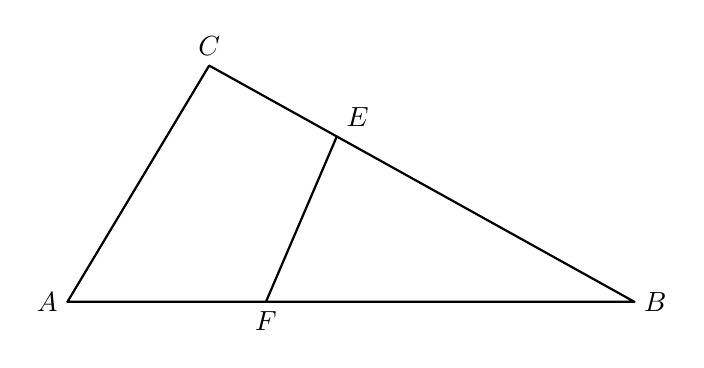
\begin{tikzpicture}[line join=round, line cap=round, >=stealth, scale=1.2]
    % 1. 定义顶点坐标 (根据图像比例估算)
    \coordinate (A) at (0,0);
    \coordinate (B) at (6,0);
    \coordinate (C) at (1.5,2.5);
    
    % 2. 定义内部点 E 和 F
    % E 在 BC 上，约在 BC 的中点偏上位置
    \coordinate (E) at ($(B)!0.7!(C)$); 
    % F 在 AB 上，约在 AB 的中点偏左位置
    \coordinate (F) at ($(A)!0.35!(B)$);

    % 3. 绘制三角形主体
    \draw[thick] (A) -- (B) -- (C) -- cycle;

    % 4. 绘制内部连接线段 EF
    \draw[thick] (E) -- (F);

    % 5. 标注顶点和各点名称
    % left, right, above, below 用于微调标签位置，保证不被线段遮挡
    \node[left] at (A) {$A$};
    \node[right] at (B) {$B$};
    \node[above] at (C) {$C$};
    \node[above right] at (E) {$E$};
    \node[below] at (F) {$F$};

    % (可选) 如果需要标注点的小圆点，可以取消下面代码的注释
    %\foreach \p in {A,B,C,E,F} \fill (\p) circle (1.5pt);

\end{tikzpicture}
\end{document}